%%%%%%%%%%%%%%%%%%%%%%%%%%%%%%%%%%%%
% Slide options
%%%%%%%%%%%%%%%%%%%%%%%%%%%%%%%%%%%%

% Option 1: Slides with solutions

\documentclass[t,compress,mathserif]{beamer}
\newcommand{\soln}[1]{\textit{#1}}
\newcommand{\solnGr}[1]{#1}

% Option 2: Handouts without solutions

%\documentclass[11pt,containsverbatim,handout]{beamer}
%\usepackage{pgfpages}
%\pgfpagesuselayout{4 on 1}[letterpaper,landscape,border shrink=5mm]
%\newcommand{\soln}[1]{ }
%\newcommand{\solnGr}{ }


%%%%%%%%%%%%%%%%%%%%%%%%%%%%%%%%%%%%
% Style
%%%%%%%%%%%%%%%%%%%%%%%%%%%%%%%%%%%%

\def\chp5@path{../../Chp 5}
\input{../../lec_style.tex}


%%%%%%%%%%%%%%%%%%%%%%%%%%%%%%%%%%%%
% Preamble
%%%%%%%%%%%%%%%%%%%%%%%%%%%%%%%%%%%%

\title[Lecture 15]{MA213: Lecture 15}
\subtitle{Module 3: Foundations for inference}
\author{OpenIntro Statistics, 4th Edition}
\institute{$\:$ \\ {\footnotesize Based on slides developed by Mine \c{C}etinkaya-Rundel of OpenIntro. \\
The slides may be copied, edited, and/or shared via the \webLink{http://creativecommons.org/licenses/by-sa/3.0/us/}{CC BY-SA license.} \\
Some images may be included under fair use guidelines (educational purposes).}}
\date{}


%%%%%%%%%%%%%%%%%%%%%%%%%%%%%%%%%%%%
% Begin document
%%%%%%%%%%%%%%%%%%%%%%%%%%%%%%%%%%%%

\begin{document}


%%%%%%%%%%%%%%%%%%%%%%%%%%%%%%%%%%%%
% Title page
%%%%%%%%%%%%%%%%%%%%%%%%%%%%%%%%%%%%

{
\addtocounter{framenumber}{-1} 
{\removepagenumbers 
\usebackgroundtemplate{\includegraphics[width=\paperwidth]{../../OpenIntro_Grid_4_3-01.jpg}}
\begin{frame}

\hfill \includegraphics[width=20mm]{../../oiLogo_highres}

\titlepage

\end{frame}
}
}


%%%%%%%%%%%%%%%%%%%%%%%%%%%%%%%%%%%%
% Sections
%%%%%%%%%%%%%%%%%%%%%%%%%%%%%%%%%%%%


%%%%%%%%%%%%%%%%%%%%%%%%%%%%%%%%%%%%
% Recap/Agenda 
%%%%%%%%%%%%%%%%%%%%%%%%%%%%%%%%%%%%
% TODO better formatting
\begin{frame}
    \frametitle{Lecture 15: Agenda}
    \begin{itemize}
        \item \hl{Previously: }Probability distributions and random variables (Chapter 4)
        \item \hl{This time: }Point estimates and sampling variability (Chapter 5.1)
        \item \hl{Reading: }Chapter 5.2 for next time
        \item \hl{Deadlines/Announcements: }HW 2.3 due today, Q1 retake in discussions
    \end{itemize}
    
\end{frame}
    

\begin{frame}
    \frametitle{Module 3: Foundations for inference}

    Up until now, we have talked about:
    \begin{itemize}
        \item \hl{Module 1. }Exploratory Data Analysis and Study Design
        \begin{itemize}
            \item Often we don't have access to a whole \hl{population} of interest, so we draw a random \hl{sample}
            \item A \hl{sample statistic} is a value computed from a data sample, like a sample mean
        \end{itemize}
        \pause
        \item \hl{Module 2. }Probability, Random Variables, and Distributions
        \begin{itemize}
            \item We use probability theory to model \hl{random experiments}, like drawing a random sample from a population
            \item The parameters of the models are called \hl{population parameters}
        \end{itemize}
    \end{itemize}
   
    \pause
    \begin{center}
        How can we use \hl{sample statistics} to learn about \hl{population parameters}?\\
        \hl{Module 3. }Foundations for inference
    \end{center}
\end{frame}

%%%%%%%%%%%%%%%%%%%%%%%%%%%%%%%%%%%%

\section{Point estimates and sampling variability (Ch. 5.1)}

%%%%%%%%%%%%%%%%%%%%%%%%%%%%%%%%%%%%

\begin{frame}
    \frametitle{Point estimates and error}

    \begin{itemize}

        \item We are often interested in \hl{population parameters}.
        \item Complete populations are difficult to collect data on, so we use \hl{sample statistics} as \hl{point estimates} for the unknown population parameters of interest.
        \item \hl{Error} in the estimate = difference between population parameter and sample statistic
        \item \hl{Bias} is systematic tendency to over- or under-estimate the true population parameter.
        \item \hl{Sampling error} describes how much an estimate will tend to vary from one sample to the next.
        \item Much of statistics is focused on understanding and quantifying sampling error, and \hl{sample size} is helpful for quantifying this error.

    \end{itemize}

\end{frame}

%%%%%%%%%%%%%%%%%%%%%%%%%%%%%%%%

%%%%%%%%%%%%%%%%%%%%%%%%%%%%%%%%%%%

\begin{frame}
    \frametitle{}
    
    \dq{Suppose we randomly sample 1,000 adults from each state in the US. Would you expect the sample means of their heights to be the same, somewhat different, or very different?}
    
    \pause
    
    \soln{Not the same, but only somewhat different.}
    
\end{frame}

%%%%%%%%%%%%%%%%%%%%%%%%%%%%%%%%%%%%

\subsection{Understanding the variability of a point estimate}

%%%%%%%%%%%%%%%%%%%%%%%%%%%%%%%%%%%%

\begin{frame}
    \frametitle{}
    
    \begin{center}
    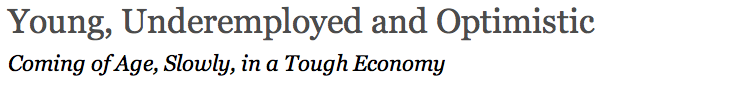
\includegraphics[width=0.95\textwidth]{\chp5@path/5-1_point_est_sampling_var/figures/pew/pew1} \\
    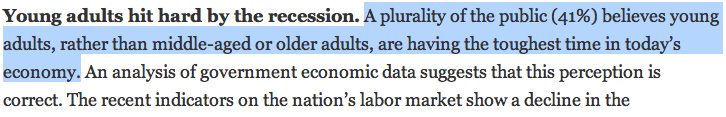
\includegraphics[width=0.95\textwidth]{\chp5@path/5-1_point_est_sampling_var/figures/pew/pew2} \\
    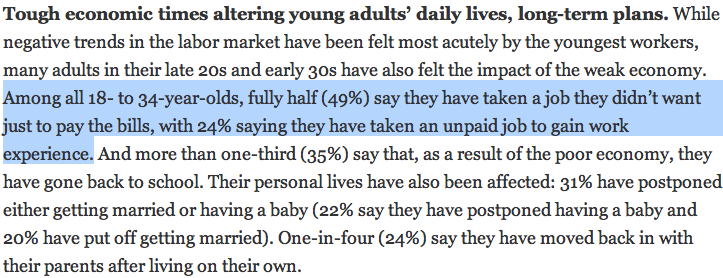
\includegraphics[width=0.95\textwidth]{\chp5@path/5-1_point_est_sampling_var/figures/pew/pew3}
    \end{center}
    
    \ct{\webURL{http://pewresearch.org/pubs/2191/young-adults-workers-labor-market-pay-careers-advancement-recession}}
    
\end{frame}

%%%%%%%%%%%%%%%%%%%%%%%%%%%%%%%%%%%%

\begin{frame}
    \frametitle{Margin of error}
    
    \begin{center}
    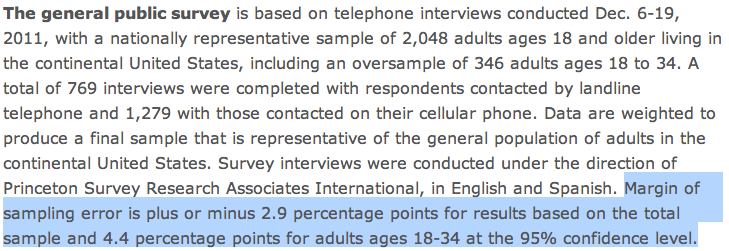
\includegraphics[width=0.95\textwidth]{\chp5@path/5-1_point_est_sampling_var/figures/pew/pew4}
    \end{center}
    
    \begin{itemize}
    
    \item 41\% $\pm$ 2.9\%: We are 95\% confident that 38.1\% to 43.9\% of the public believe young adults, rather than middle-aged or older adults, are having the toughest time in today's economy.
    
    \item 49\% $\pm$ 4.4\%: We are 95\% confident that 44.6\% to 53.4\% of 18-34 years olds have taken a job they didn't want just to pay the bills.
    
    \end{itemize}
    
\end{frame}

%%%%%%%%%%%%%%%%%%%%%%%%%%%%%%%%%%%

\begin{frame}
    \frametitle{}
    
    \dq{Suppose the proportion of American adults who support the expansion of solar energy is p = 0.88, which is our parameter of interest. Is a randomly selected American adult more or less likely to support the expansion of solar energy?}
    
    \pause
    
    \soln{More likely.}
    
\end{frame}

%%%%%%%%%%%%%%%%%%%%%%%%%%%%%%%%

\begin{frame}
    \frametitle{}
    
    \dq{Suppose that you don't have access to the population of all American adults, which is a quite likely scenario. In order to estimate the proportion of American adults who support solar power expansion, you might sample from the population and use your sample proportion as the best guess for the unknown population proportion.}
    
    \begin{itemize}
    
    \item Sample, with replacement, 1000 American adults from the population, and record whether they support or not solar power expansion.
    
    \item Find the sample proportion.
    
    \item Plot the distribution of the sample proportions obtained by members of the class.
    
    \end{itemize}
    
\end{frame}
    
%%%%%%%%%%%%%%%%%%%%%%%%%%%%%%%%%%

\section{R Demo: Sampling distributions}

%%%%%%%%%%%%%%%%%%%%%%%%%%%%%%%%%%

\begin{frame}
    \frametitle{Sampling distributions are never observed}

    \begin{itemize}

        \item In real-world applications, we never actually observe the sampling distribution, yet it is useful to always think of a point estimate as coming from such a hypothetical distribution.
        \item Understanding the sampling distribution will help us characterize and make sense of the point estimates that we do observe.

    \end{itemize}

\end{frame}

%%%%%%%%%%%%%%%%%%%%%%%%%%%%%%%%

%%%%%%%%%%%%%%%%%%%%%%%%%%%%%%%%

\section{Edfinity quiz}

%%%%%%%%%%%%%%%%%%%%%%%%%%%%%%%%

\begin{frame}
    \frametitle{Edfinity Quiz}

    \begin{itemize}

        \item If the population proportion were 0.2 and the sample size were 100:
        \begin{itemize}
            \item Where would you expect the middle of the sampling distribution to be?
            \item Would the sampling distribution be symmetrical?
            \item Would the sampling distribution be wider/narrower/the same?
        \end{itemize}
        \item If the population proportion were 0.99 and the sample size were 100:
        \begin{itemize}
            \item Where would you expect the middle of the sampling distribution to be?
            \item Would the sampling distribution be symmetrical?
            \item Would the sampling distribution be wider/narrower/the same?
        \end{itemize}
 
    \end{itemize}

\end{frame}

\begin{frame}
    \frametitle{Edfinity Quiz}
    \begin{center}
        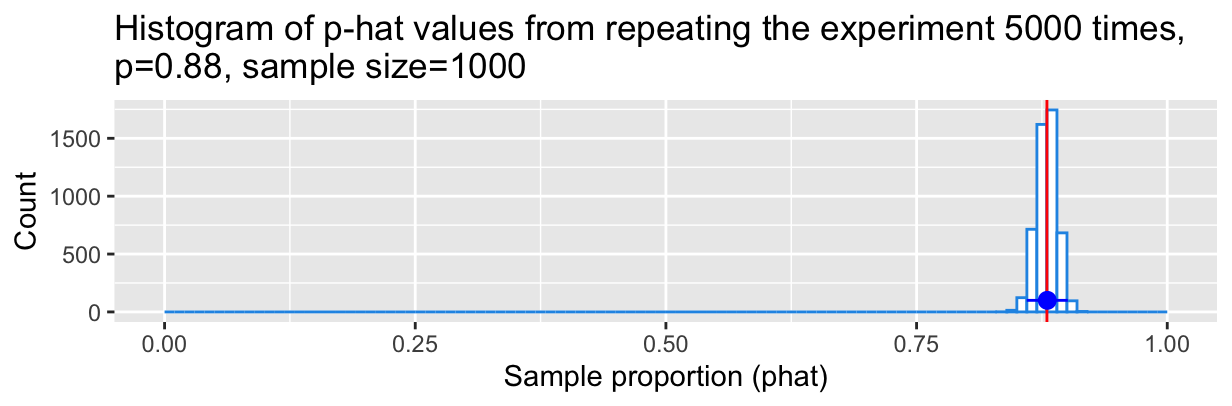
\includegraphics[width=0.75\textwidth]{sampling_distribution.png}
    \end{center}
    
    \begin{table}[h!]
        \centering
        \begin{tabular}{|c|c|c|c|}
        \hline
         & Middle? & Symm? & Wider/Narrower/Same? \\ 
        \hline
        p=0.88, n=1000 & $\sim0.88$ & Yes & Same \\ 
        \hline
        p=0.2, n=100 &  &  &  \\ 
        \hline
        p=0.99, n=100 &  &  &  \\ 
        \hline
        \end{tabular}
    \end{table}
\end{frame}

\begin{frame}
    \frametitle{Edfinity Quiz}
    What would happen if the sample size were 10?
\end{frame}

%%%%%%%%%%%%%%%%%%%%%%%%%%%%%%%%%%

\section{R Demo: What would happen if...}

%%%%%%%%%%%%%%%%%%%%%%%%%%%%%%%%

\section{Board work: Deriving theoretical sampling distribution in the Binomial case}

%%%%%%%%%%%%%%%%%%%%%%%%%%%%%%%%%%

\begin{frame}
    \frametitle{Rule of succession}

    There can be multiple statistics that estimate the same population parameter
    \begin{itemize}

        \item \hl{The Rule Of Succession} (Laplace, 18th Century)
        \item What is the probability that the sun will rise tomorrow, given that it has risen every day for the last 5000 years?
        \item 0 is an unsatisfying answer
        \item Approach: Pretend we have seen one success and one failure
    
    \end{itemize}

    Sample proportion:
     \begin{align}
        \hat{p}=\frac{k}{n}
    \end{align}
 
    Rule of Succession:
    \begin{align}
        \hat{p}^*=\frac{k +1}{n+2}
    \end{align}
 
\end{frame}


%%%%%%%%%%%%%%%%%%%%%%%%%%%%%%%%%%%%

\section{R Demo: Comparing different estimators based on their sampling distributions}

%%%%%%%%%%%%%%%%%%%%%%%%%%%%%%%%
% End document
%%%%%%%%%%%%%%%%%%%%%%%%%%%%%%%%%%%%

\end{document}